\documentclass[tikz,border=6pt]{standalone}
\usepackage{amsmath,amssymb,bm}
\usetikzlibrary{positioning,fit,calc,arrows.meta}

\begin{document}
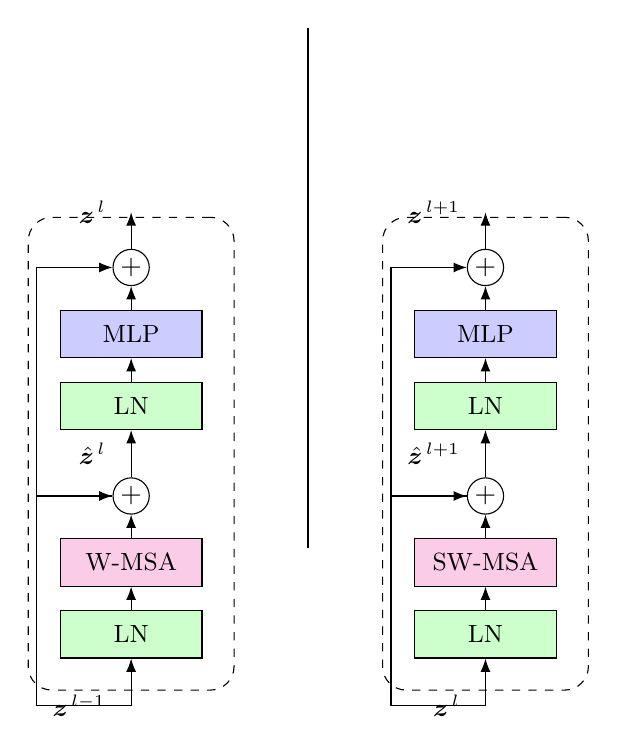
\begin{tikzpicture}[
  font=\small,
  >=Latex,
  box/.style={draw, minimum width=18mm, minimum height=6mm, align=center},
  mlp/.style={box, fill=blue!20},
  ln/.style={box, fill=green!20},
  msa/.style={box, fill=magenta!20},
  add/.style={draw, circle, inner sep=0pt, minimum size=4.6mm, font=\normalsize},
  dashedbox/.style={draw, dashed, rounded corners=3mm, inner sep=4mm}
]

% =========================
% Left block (W-MSA)
% =========================
\coordinate (l_in) at (0,0);

\node[ln,  above=6mm of l_in] (l_ln1) {LN};
\node[msa, above=3mm of l_ln1] (l_msa) {W-MSA};
\node[add, above=3mm of l_msa] (l_add1) {$+$};

\node[ln,  above=6mm of l_add1] (l_ln2) {LN};
\node[mlp, above=3mm of l_ln2] (l_mlp) {MLP};
\node[add, above=3mm of l_mlp] (l_add2) {$+$};

\coordinate (l_out) at ($(l_add2)+(0,7mm)$);

% main path
\draw[->] (l_in) -- (l_ln1);
\draw[->] (l_ln1) -- (l_msa);
\draw[->] (l_msa) -- (l_add1);

\draw[->] (l_add1) -- (l_ln2) node[midway,left=2mm] {$\hat{\bm z}^{\,l}$};
\draw[->] (l_ln2) -- (l_mlp);
\draw[->] (l_mlp) -- (l_add2);
\draw[->] (l_add2) -- (l_out);

% labels
\node[left=2mm of l_in]  {$\bm z^{\,l-1}$};
\node[left=2mm of l_out] {$\bm z^{\,l}$};

% residuals
\draw[->] (l_in) -- ++(-12mm,0) |- (l_add1.west);
\draw[->] (l_add1) -- ++(-12mm,0) |- (l_add2.west);

% dashed frame
\node[dashedbox, fit=(l_ln1)(l_add2)] (l_frame) {};

% =========================
% Right block (SW-MSA)
% =========================
\coordinate (r_in) at (45mm,0);

\node[ln,  above=6mm of r_in] (r_ln1) {LN};
\node[msa, above=3mm of r_ln1] (r_msa) {SW-MSA};
\node[add, above=3mm of r_msa] (r_add1) {$+$};

\node[ln,  above=6mm of r_add1] (r_ln2) {LN};
\node[mlp, above=3mm of r_ln2] (r_mlp) {MLP};
\node[add, above=3mm of r_mlp] (r_add2) {$+$};

\coordinate (r_out) at ($(r_add2)+(0,7mm)$);

% main path
\draw[->] (r_in) -- (r_ln1);
\draw[->] (r_ln1) -- (r_msa);
\draw[->] (r_msa) -- (r_add1);

\draw[->] (r_add1) -- (r_ln2) node[midway,left=2mm] {$\hat{\bm z}^{\,l+1}$};
\draw[->] (r_ln2) -- (r_mlp);
\draw[->] (r_mlp) -- (r_add2);
\draw[->] (r_add2) -- (r_out);

% labels
\node[left=2mm of r_in]  {$\bm z^{\,l}$};
\node[left=2mm of r_out] {$\bm z^{\,l+1}$};

% residuals
\draw[->] (r_in) -- ++(-12mm,0) |- (r_add1.west);
\draw[->] (r_add1) -- ++(-12mm,0) |- (r_add2.west);

% dashed frame
\node[dashedbox, fit=(r_ln1)(r_add2)] (r_frame) {};

% =========================
% Divider line
% =========================
\draw[line width=0.6pt] ($(l_frame.east)!0.5!(r_frame.west)+(0,-12mm)$)
  -- ($(l_frame.east)!0.5!(r_frame.west)+(0,54mm)$);

\end{tikzpicture}
\end{document}
